\section{\label{sec:init-pair-distribution} Pair distribution function}
The $n$-particle distribution function is defined via the $n$-particle densities as follows (for reference, see Section~2.6 in~\cite{HansenMcDonald13})
\begin{equation*}
	\label{def:g_n}
	g^{(n)}({\vb r}_1, \dotsc, {\vb r}_n)=\frac{\rho^{(n)}({\vb r}_1, \dotsc, {\vb r}_n)}{\prod_{i=1}^{n}\rho^{(1)}({\vb r}_i)}
\end{equation*}
where the $n$-particle density defined in the grand canonical ensemble is
\begin{eqnarray*}
	\label{def:rho_n}
	\rho^{(n)}({\vb r}_1, \dotsc ,{\vb r}_n) = \frac{1}{\Xi}\sum_{N=n}^{\infty} \frac{\zeta^N}{(N-n)!} \int\exp(-\beta W_{N_v}(\gamma_N)) {\rm d} {\vb r}_{n+1} \dotsc {\rm d} {\vb r}_N.
\end{eqnarray*}
In this work, our goal is to calculate the pair distribution function $g^{(2)}({\vb r}_1, {\vb r}_2)$
\begin{equation*}
	g^{(2)}({\vb r}_1, {\vb r}_2) = \frac{\rho^{(2)}({\vb r}_1, {\vb r}_2)}{\rho^{(1)}({\vb r}_1) \rho^{(1)}({\vb r}_2)}.
\end{equation*}
Therefore, we first need to calculate the one- and two-particle densities.

\subsection{One-particle density}

Let us first calculate $\rho^{(1)}$. By definition
\begin{equation}
	\label{def:rho1}
	\rho^{(1)} ({\vb r}_1) = \Xi^{-1} \sum_{N=1}^{\infty} \frac{\zeta^N}{(N-1)!} \int \exp(-\beta W_{N_v}({\vb r}_1, \dotsc, {\vb r}_N)) {\rm d} {\vb r}_2 \dotsc {\rm d} {\vb r}_N.
\end{equation}
Applying the method described in~\cite{KKD20}, we obtain the following result
\begin{equation*}
	\rho^{(1)} ({\vb r}_1) = \frac{K_1(T^*, \mu^*; \bar{y}_{\rm max})}{v K_0(T^*,\mu^*; \bar{y}_{\rm max})} = \frac{\rho^*(T^*,\mu^*)}{v}
\end{equation*}
where we used the following equality~\cite[Eq.~(42)]{RDKPS25arxiv}
\begin{equation}
	\label{eq:rho_in_y}
	\rho^* = \frac{K_1(T^*, \mu^*; \bar{y}_{\rm max})}{K_0(T^*,\mu^*; \bar{y}_{\rm max})}.
\end{equation}
Therefore, for the considered cell fluid model with Curie-Weiss interaction we obtained the result known for homogeneous systems: the single-particle density is equal to the average particle density, see~\cite[Eq.~(2.6.5)]{HansenMcDonald13}:
\begin{equation}
	\rho^{(1)}({\vb r}_1) = \rho.
\end{equation}

In the presented theory, the average value of the cell occupation number can also be calculated using the probability measure $Q_{T^*,\mu^*}(n)$~\cite{KKD20}:
\begin{equation*}
	Q_{T^*,\mu^*}(n) = \frac{1}{K_0(T^*, \mu^*; \bar{y}_{\rm max}) n!} \left(v^* T^{*3/2}\right)^n \exp\left[\left(\bar{y}_{\rm max} + \frac{\mu^*}{T^*} \right)n - \frac{a}{2T^*}n^2 \right],
	\quad n \in \mathbb{N}_0,
\end{equation*}
so that
\begin{equation*}
	\langle n \rangle_{Q} = \sum_{n=0}^{\infty} n Q_{T^*, \mu^*}(n).
\end{equation*}
Hence, we can write the following equalities:
\begin{equation}
	v \rho^{(1)}({\vb r}_1) = \langle n \rangle_{Q} = \rho^*.
\end{equation}

\subsection{Two-particle density}

Let us now calculate the two-particle density, defined as
\begin{equation*}
	\rho^{(2)} ({\vb r}_1, {\vb r}_2) = \Xi^{-1} \sum_{N=2}^{\infty} \frac{\zeta^N}{(N-2)!} \int \exp(-\beta W_{N_v}({\vb r}_1, {\vb r}_2, \dotsc, {\vb r}_N)) {\rm d} {\vb r}_3 \dotsc {\rm d} {\vb r}_N.
\end{equation*}
To deal with this expression, we again follow the methodology developed in~\cite{KKD20}. However, it is important to note that the result for $\rho^{(2)}({\vb r}_1, {\vb r}_2)$ varies depending on whether ${\vb r}_1$ and ${\vb r}_2$ belong to the same cell or to different cells.

When ${\vb r}_1$ and ${\vb r}_2$ belong to different cells, the result for $\rho^{(2)}({\vb r}_1, {\vb r}_2)$ is as follows
\begin{eqnarray}
	\rho^{(2)} ({\vb r}_1, {\vb r}_2) & = & \left[\frac{K_1(T^*, \mu^*; \bar{y}_{\rm max})}{v K_0(T^*, \mu^*; \bar{y}_{\rm max})}\right]^2
	\nonumber \\
	& = & \frac{\rho^{*2}}{v^2} = \frac{\langle n \rangle_{Q}^2}{v^2}.
\end{eqnarray}
From this expression the result for $g^{(2)}({\vb r}_1, {\vb r}_2)$ follows immediately
\begin{equation}
	\label{g2_diff}
	g^{(2)}({\vb r}_1, {\vb r}_2) = 1, \quad \text{if } \nexists \Delta_l ({\vb r}_1, {\vb r}_2 \in \Delta_l),
\end{equation}
that is, when ${\vb r}_1$ and ${\vb r}_2$ belong to different cells.

When ${\vb r}_1$ and ${\vb r}_2$ belong to the same cell, the result for $\rho^{(2)}({\vb r}_1, {\vb r}_2)$ is as follows
\footnote{compare with Eq.~(2.6.4) from~\cite{HansenMcDonald13}}
\begin{equation}
	\rho^{(2)}({\vb r}_1, {\vb r}_2) = \frac{1}{v^2} \sum_{n=0}^{\infty} n(n-1) Q_{T^*, \mu^*}(n) 
	= \frac{\langle n(n-1) \rangle_{Q}}{v^2}.
\end{equation}
and for $g^{(2)}({\vb r}_1, {\vb r}_2)$ one gets
\begin{equation}
	\label{g2_same}
	g^{(2)}({\vb r}_1, {\vb r}_2) = \frac{\langle n(n-1) \rangle_{Q}}{\langle n \rangle_{Q}^2}, \quad \text{if } \exists \Delta_l ({\vb r}_1, {\vb r}_2 \in \Delta_l),
\end{equation}
that is, when both ${\vb r}_1$ and ${\vb r}_2$ belong to the same cell $\Delta_l$. Based on Eqs.~\eqref{g2_diff} and~\eqref{g2_same}, the general expression for $g^{(2)}({\vb r}_1, {\vb r}_2)$ takes on the form
\begin{equation}
	g^{(2)}({\vb r}_1, {\vb r}_2) =  \left\{
	\begin{array}{ll}
		1, & \text{if } \nexists \Delta_l ({\vb r}_1, {\vb r}_2 \in \Delta_l),
		\\
		\frac{\langle n(n-1) \rangle_{Q}}{\langle n \rangle_{Q}^2}, & \text{if } \exists \Delta_l ({\vb r}_1, {\vb r}_2 \in \Delta_l).
	\end{array}
	\right.
\end{equation} 

In what follows, we will mostly focus on $g^{(2)}({\vb r}_1, {\vb r}_2)$ with ${\vb r}_1$ and ${\vb r}_2$ in the same cell.
First thing to note is that given ${\vb r}_1$ and ${\vb r}_2$ belong to the same cell, the two-particle density does not otherwise depend on the position of the particles, thus we can just write $\rho^{(2)}$ for simplicity. The same consequently applies to $g^{(2)}$.

Before proceeding with numerical and graphical results for the pair distribution function $g^{(2)}$ let us first rewrite it in a few alternative representations.

If expressed in terms of $K_j$, $\rho^{(2)}$ and $g^{(2)}$ take on the following forms:
\begin{eqnarray}
	\rho^{(2)} = \frac{K_2(T^*, \mu^*; \bar{y}_{\rm max}) - K_1(T^*, \mu^*; \bar{y}_{\rm max})}{v^2 K_0(T^*, \mu^*; \bar{y}_{\rm max})},
\end{eqnarray}
and
\begin{eqnarray}
	g^{(2)} & = & \frac{\left[K_2(T^*, \mu^*; \bar{y}_{\rm max}) - K_1(T^*, \mu^*; \bar{y}_{\rm max})\right] K_0(T^*, \mu^*; \bar{y}_{\rm max})}{K_1(T^*, \mu^*; \bar{y}_{\rm max})^2},
\end{eqnarray}
respectively.

We can represent the results for the pair distribution function in the form of parametric equations. Applying the idea taken from~\cite{KD22}, we introduce a new function
\begin{equation}
	\label{eq:change_y_to_z}
	\bar{z}_{\rm max} = \bar{y}_{\rm max} + \frac{\mu^*}{T^*},
\end{equation}
and express the chemical potential as a function of two variables $(T^*, \bar{z}_{\rm max})$
\begin{equation}
	\label{eq:mu_in_z}
	\mu^* = T^* \bar{z}_{\mathrm{max}} - \frac{\tilde{K}_1(T^*;\bar{z}_{\mathrm{max}})}{\tilde{K}_0(T^*;\bar{z}_{\mathrm{max}})},
\end{equation}
where the special functions $\tilde{K}_j$ are written as
\begin{eqnarray}
	\tilde{K}_j(T^*;\bar{z}_{\mathrm{max}}) = \sum_{n=0}^{\infty} \frac{n^j (v^* T^{*3/2})^n}{n!} 
	%\nonumber\\
	%\times 
	\exp[\bar{z}_{\mathrm{max}}n - \frac{a}{2T^*}n^2].
\end{eqnarray}
Now, the two-particle density and the pair distribution function take on the following forms
\begin{equation}
	\rho^{(2)} = \frac{\tilde{K}_2(T^*; \bar{z}_{\rm max}) - \tilde{K}_1(T^*; \bar{z}_{\rm max})}{v^2 \tilde{K}_0(T^*; \bar{z}_{\rm max})},
\end{equation}
\begin{equation}
	\label{eq:g2_in_z}
	g^{(2)} = \frac{\left[\tilde{K}_2(T^*; \bar{z}_{\rm max}) - \tilde{K}_1(T^*; \bar{z}_{\rm max})\right] K_0(T^*; \bar{z}_{\rm max})}{\tilde{K}_1(T^*; \bar{z}_{\rm max})^2}.
\end{equation}
At any given temperature $T^*$, Eqs.~\eqref{eq:g2_in_z} and~\eqref{eq:mu_in_z} can be formally considered as a parametric equation for the pair distribution function $g^{(2)}$ as a function of $\mu^*$, with $\bar{z}_{\mathrm{max}}$ being the parameter.

Similarly, if Eq.~\eqref{eq:rho_in_y} is rewritten as
\begin{equation}
	\label{eq:rho_in_z}
	\rho^*(T^*;\bar{z}_{\mathrm{max}}) = \frac{\tilde{K}_1(T^*;\bar{z}_{\mathrm{max}})}{\tilde{K}_0(T^*;\bar{z}_{\mathrm{max}})},
\end{equation}
then Eqs.~\eqref{eq:g2_in_z} and~\eqref{eq:rho_in_z} constitute a parametric equation for the pair distribution function $g^{(2)}$ as a function of $\rho^*$, at any given $T^*$ and with $\bar{z}_{\mathrm{max}}$ being the parameter.

{\it III} \\
For the average value of $n$ note the following:
\begin{eqnarray*}
	K_0(\bar{z}, p) \langle n \rangle_Q & = & 
	v^{-1} \sum_{n=1}^{\infty} n \frac{v^n}{n!} \exp(\bar{z}n - \frac{ap}{2}n^2)
	\\
	& = & \sum_{n=1}^{\infty} \frac{v^{n-1}}{(n-1)!} \exp(\bar{z}n - \frac{ap}{2}n^2)
	\\
	& = & \left| n=m+1; \quad \sum_{n=1}^{\infty} \rightarrow \sum_{m=0}^{\infty}; \quad n^2 = m^2 + 2m + 1 \right|
	\\
	& = & \exp(\bar{z} - \frac{ap}{2}) \sum_{n=0}^{\infty} \frac{v^n}{n!} \exp\left[(\bar{z} - ap)n - \frac{ap}{2}n^2 \right]
	\\
	& = & \exp(\bar{z} - \frac{ap}{2}) \langle \exp(-apn) \rangle_Q
	\\
	& = & \exp(\bar{z} - \frac{ap}{2}) K_0 (\bar{z} - ap, p),
\end{eqnarray*}
and thus
\begin{equation*}
	\langle n \rangle_Q = \frac{K_0(\bar{z} - ap, p)}{K_0(\bar{z}, p)} \exp(\bar{z} - \frac{ap}{2})
\end{equation*}

For the average value of $n(n-1)$ note the following
\begin{eqnarray*}
	K_0(\bar{z}, p) \langle n(n-1) \rangle_Q & = & 
	v^{-2} \sum_{n=2}^{\infty} n(n-1) \frac{v^n}{n!} \exp(\bar{z}n - \frac{ap}{2}n^2)
	\\
	& = & \sum_{n=2}^{\infty} \frac{v^{n-2}}{(n-2)!} \exp(\bar{z}n - \frac{ap}{2}n^2)
	\\
	& = & \left| n=m+2; \quad \sum_{n=2}^{\infty} \rightarrow \sum_{m=0}^{\infty}; \quad n^2 = m^2 + 4m +4 \right|
	\\
	& = & \exp(2\bar{z} - 2ap) \sum_{n=0}^{\infty} \frac{v^n}{n!} \exp\left[(\bar{z} - 2ap)n - \frac{ap}{2}n^2 \right]
	\\
	& = & \exp(2\bar{z} - 2ap) \langle \exp(-2apn) \rangle_Q
	\\
	& = & \exp(2\bar{z} - 2ap) K_0(\bar{z} - 2ap, p),
\end{eqnarray*}
and thus
\begin{equation*}
	\langle n(n-1) \rangle_Q = \frac{K_0(\bar{z} - 2ap, p)}{K_0(\bar{z}, p)} \exp(2\bar{z} - 2ap).
\end{equation*}

The pair distribution function takes on the form
\begin{equation}
	g^{(2)} = \exp(-ap) \frac{K_0(\bar{z} - 2ap, p) K_0(\bar{z}, p)}{K_0(\bar{z}-ap, p)^2}
\end{equation}
Note that the factor $\exp(-ap)$ is the low-density limit of the pair distribution function that can be obtained from the Boltzman factor of the interaction potential, see Appendix~\ref{sec:low-dens}.

\begin{figure}[htbp]
	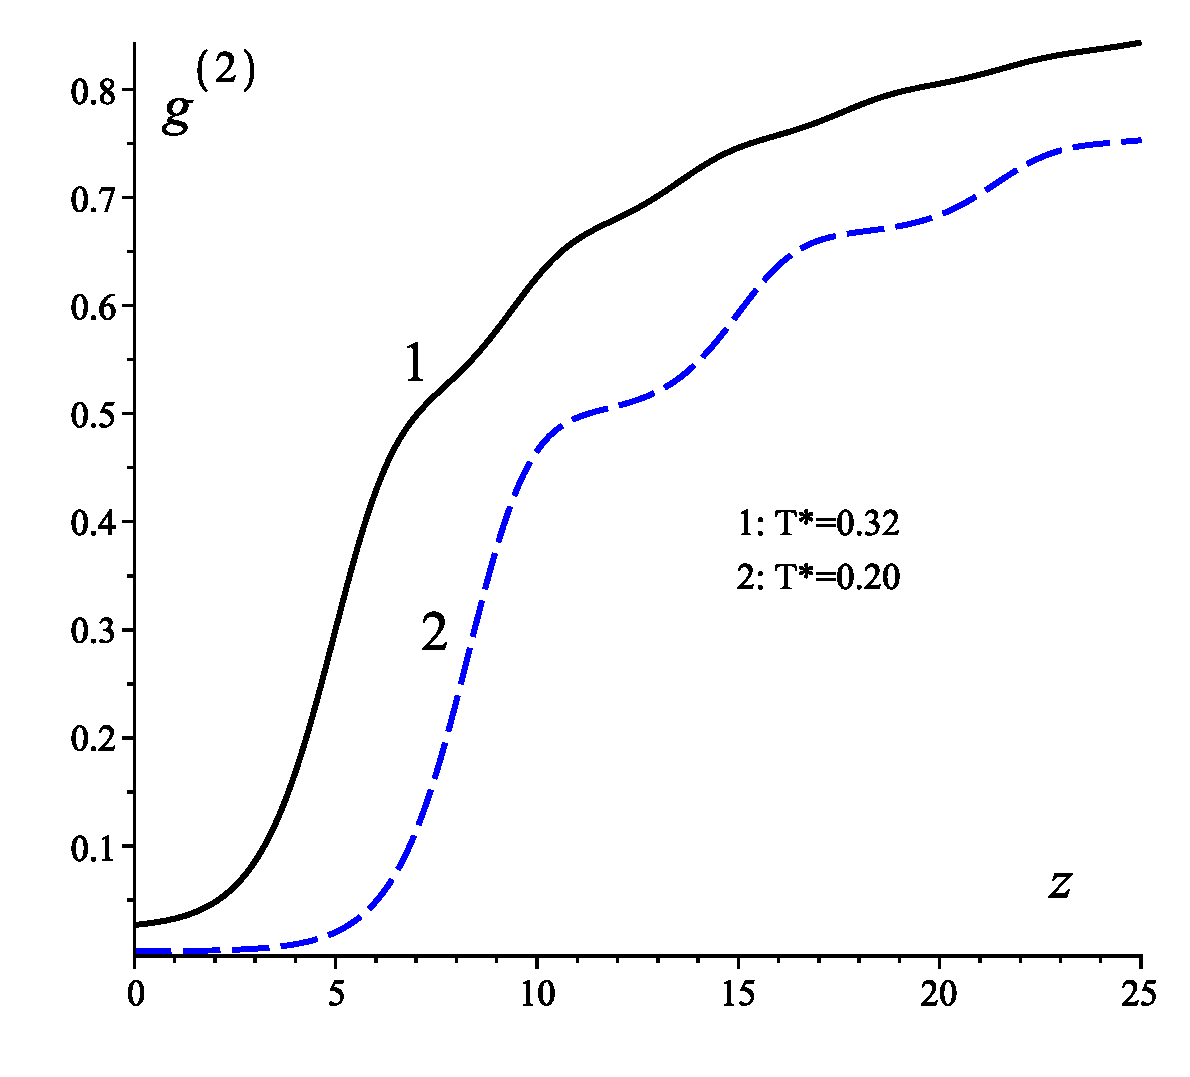
\includegraphics[width=0.7\textwidth,angle=0]{g2_vs_z}
	\caption{Pair distribution function $g^{(2)}$ versus $\bar{z}$.}
	\label{fig:g2_z}
\end{figure}
\begin{figure}[htbp]
	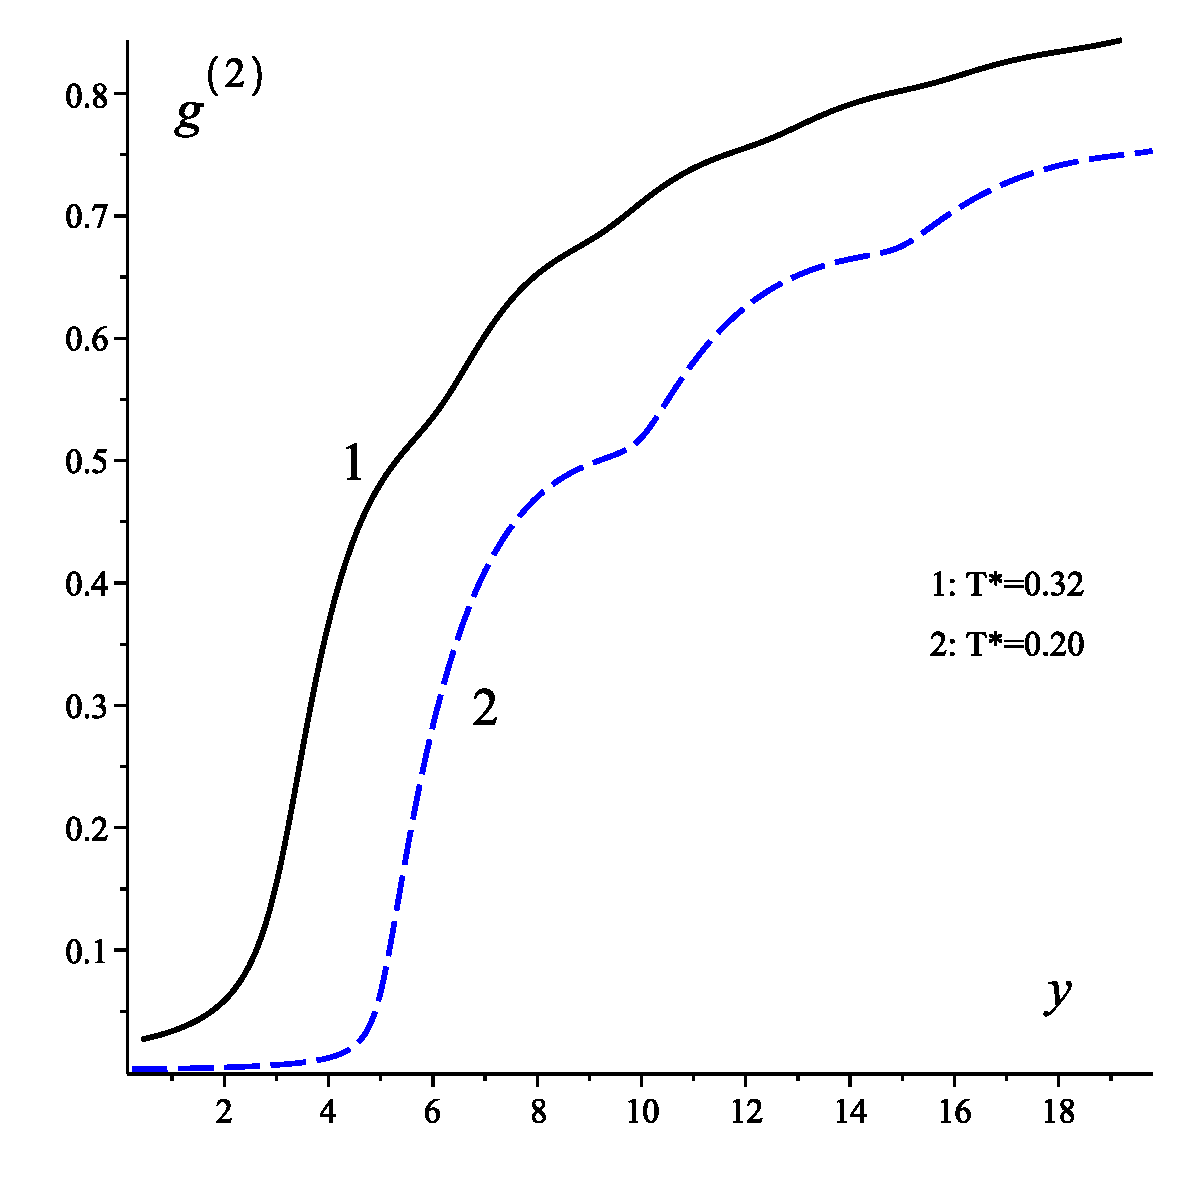
\includegraphics[width=0.7\textwidth,angle=0]{g2_vs_y}
	\caption{Pair distribution function $g^{(2)}$ versus $\bar{y}$.}
	\label{fig:g2_y}
\end{figure}

\begin{figure}[htbp]
	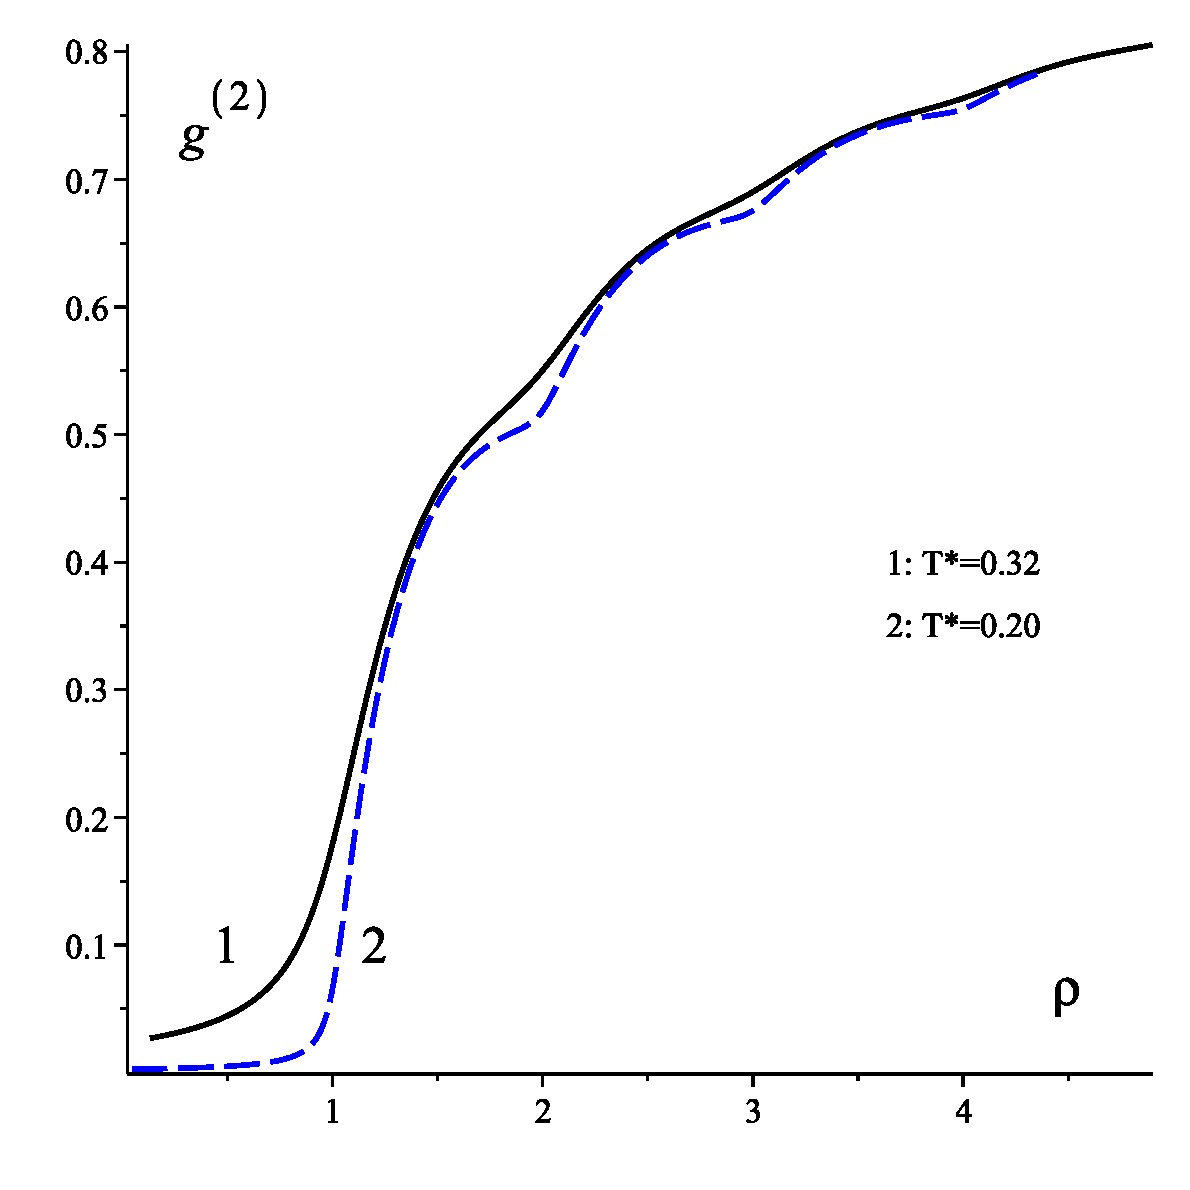
\includegraphics[width=0.7\textwidth,angle=0]{g2_vs_rho}
	\caption{Pair distribution function $g^{(2)}$ versus $\rho$.}
	\label{fig:g2_rho}
\end{figure}

\begin{figure}[htbp]
	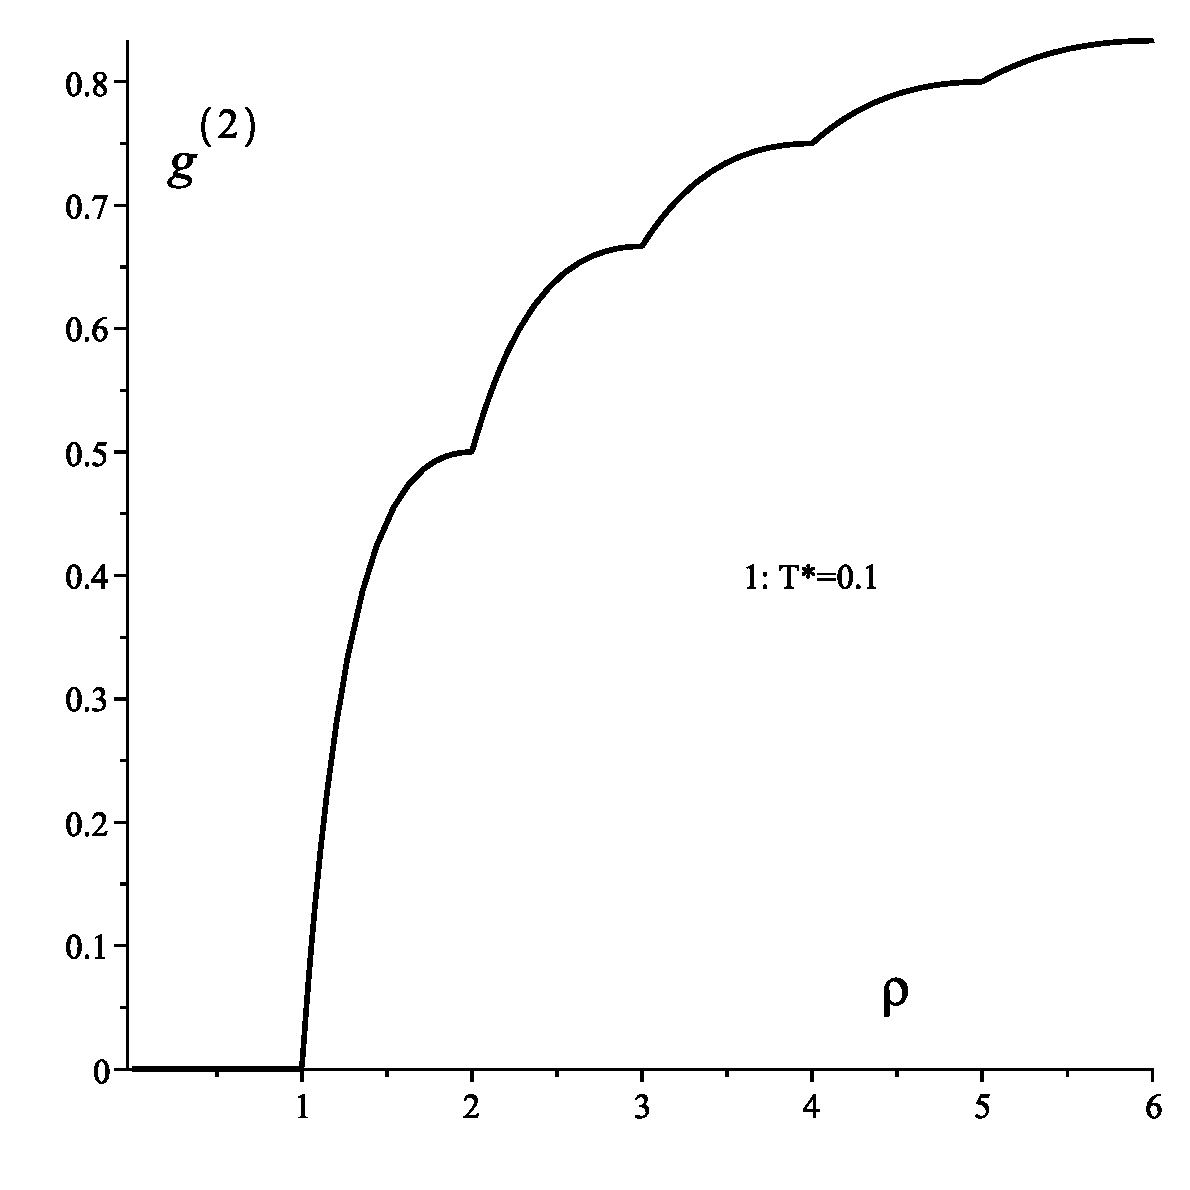
\includegraphics[width=0.7\textwidth,angle=0]{g2_vs_rho_low_temp}
	\caption{Pair distribution function $g^{(2)}$ versus $\rho$ at low temperature $T^*=0.1$.}
	\label{fig:g2_rho_low_temp}
\end{figure}

In Figure~\ref{fig:g2_z} the pair distribution function is shown as a function of $\bar{z}$ for two different values of temperature: $T^*=0.32$, which is above the range of critical temperatures, and $T^*=0.20$, which is below the range of critical temperatures. 

In Figure~\ref{fig:g2_y} the pair distribution function is shown as a function of $\bar{y}$ for the same temperatures.

In Figure~\ref{fig:g2_rho} the pair distribution function is shown as a function of density $\rho$ for the same temperatures.

Very interesting behavior of $g^{(2)}$ is observed in Figure~\ref{fig:g2_rho_low_temp}, where the dependency on density is presented in the low temperature limit, namely for $T^*=0.1$ 

The dependence of the pair distribution function on the chemical potential $\beta\mu$ is shown in Firugre~\ref{fig:g2_mu}.
\begin{figure}[htbp]
	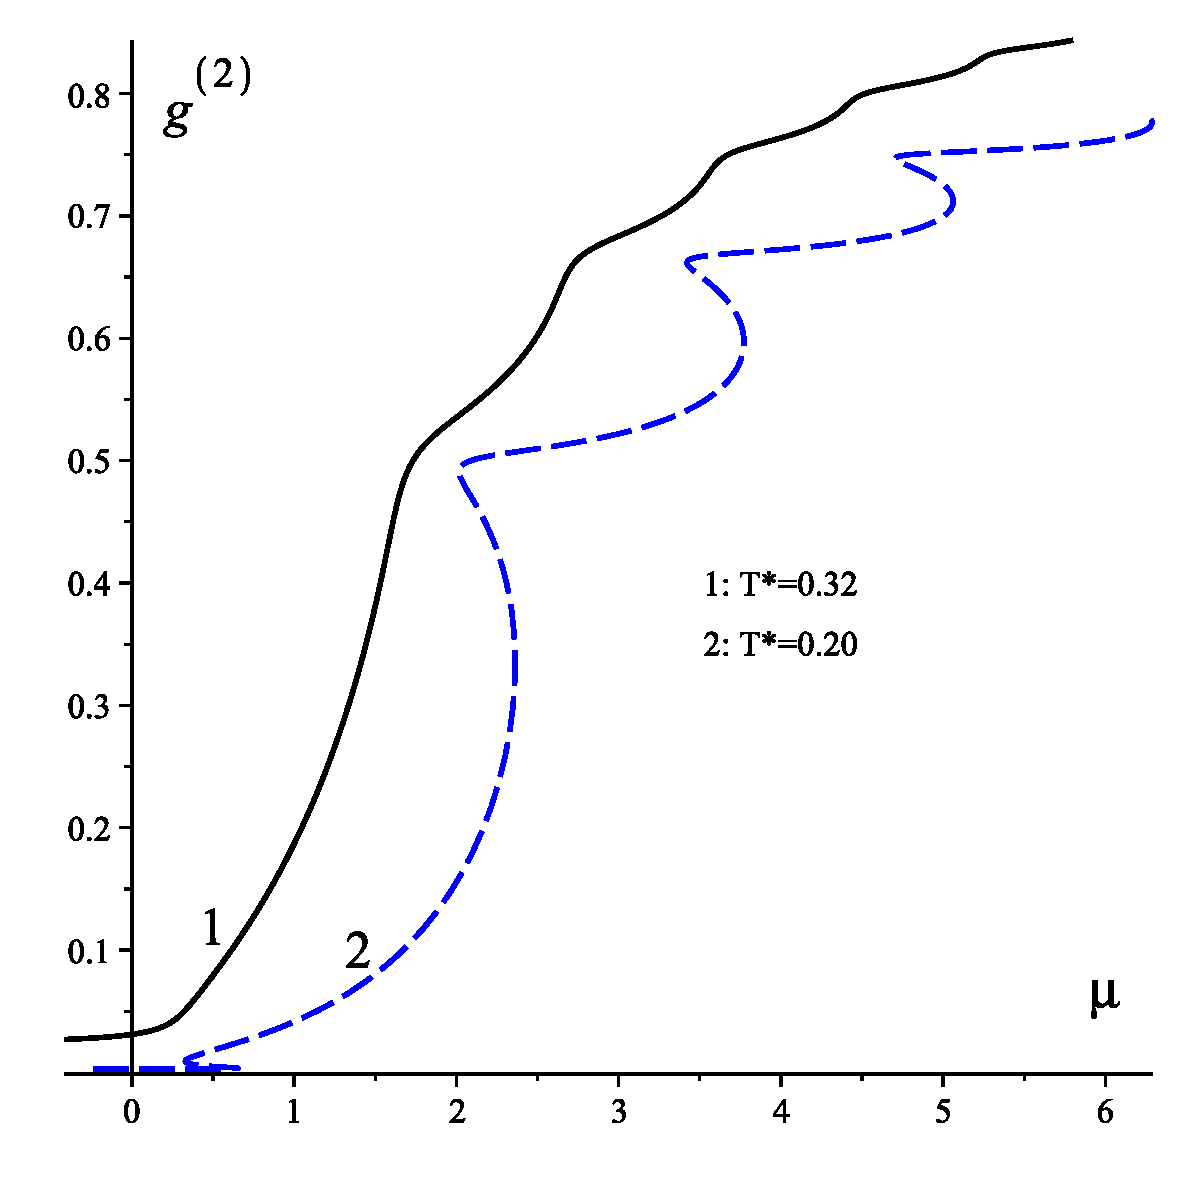
\includegraphics[width=0.7\textwidth,angle=0]{g2_vs_mu}
	\caption{Pair distribution function $g^{(2)}$ versus $\beta\mu$.}
	\label{fig:g2_mu}
\end{figure}

\begin{figure}[htbp]
	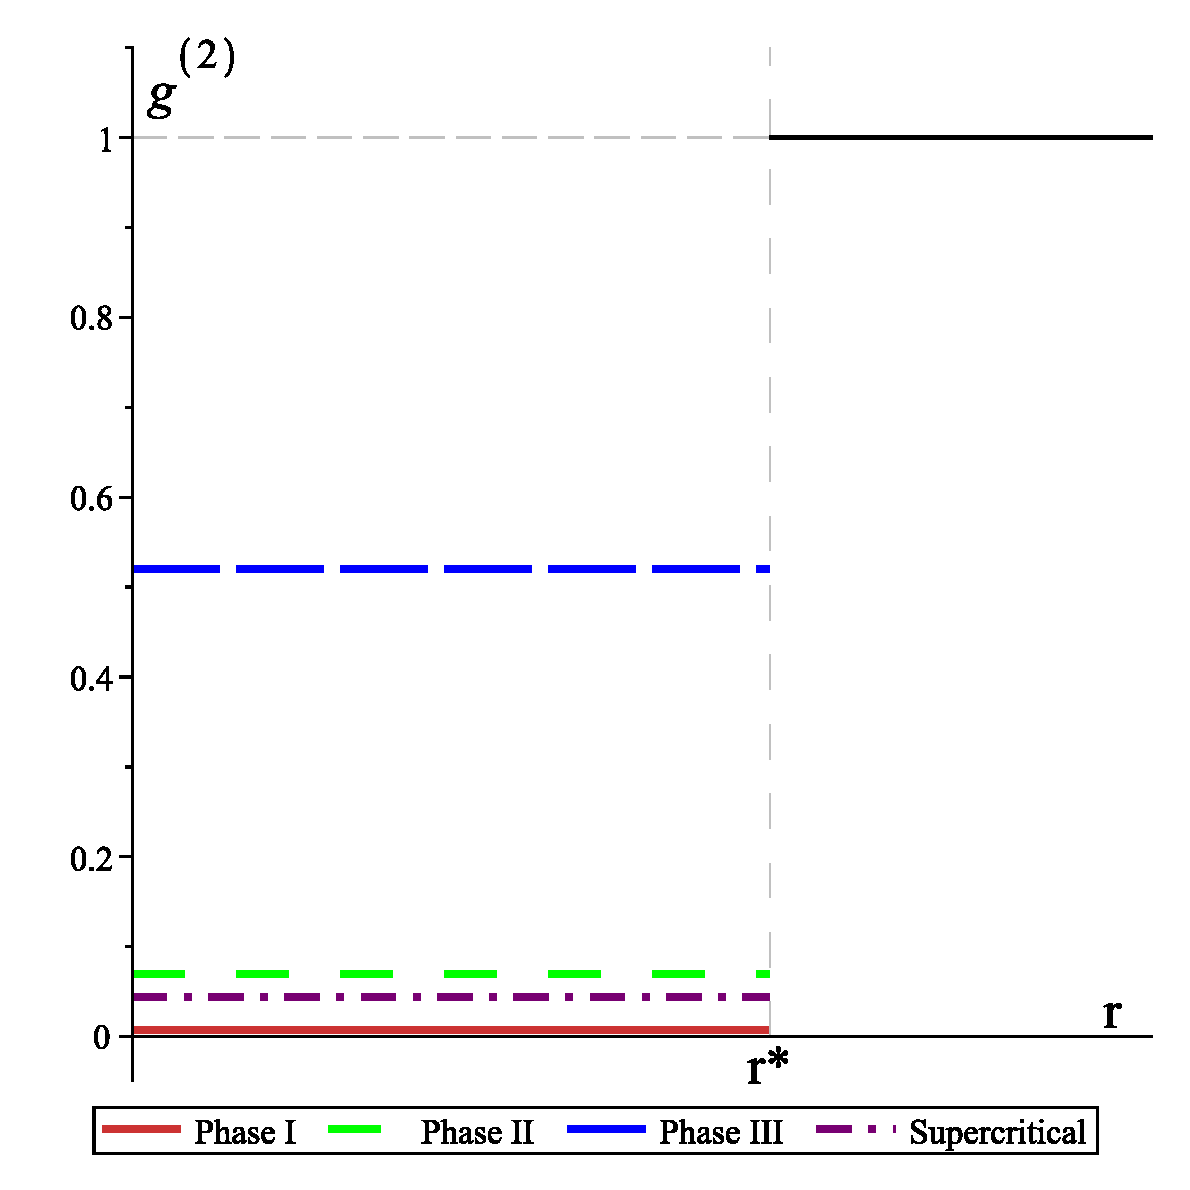
\includegraphics[width=0.6\textwidth,angle=0]{g2_vs_r}
	\caption{Pair distribution function $g^{(2)}$ as a function of separation $r$. The quantity $r^*$ denotes distance from the point with coordinate $x_1$ to the boundary of the cubic cell in the direction of $x_2$. Phase I - $T = 0.925T_c,$ $\rho^*=0.1$; Phase II - $T = 0.8T_c,$ $\rho^* = 1.0$; Phase III - $T = 0.8T_c,$ $\rho^* = 2.0$; Supercritical - $T = 1.257T_c,$ $\rho^* = 0.5$.}
	\label{fig:g2_r}
\end{figure}

\begin{figure}[htbp]
	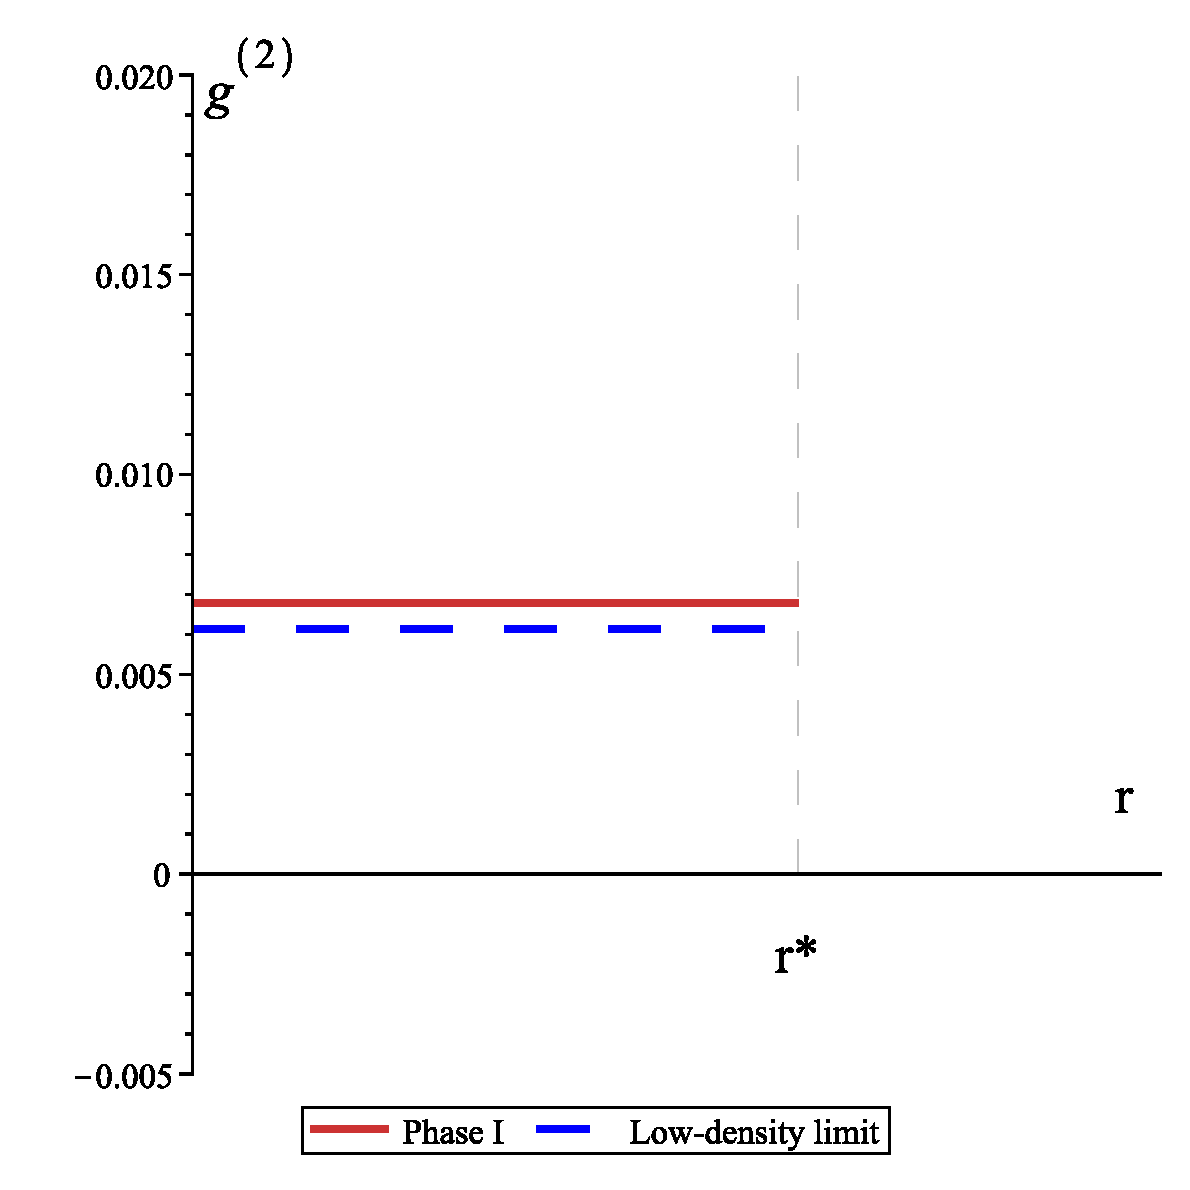
\includegraphics[width=0.6\textwidth,angle=0]{g2_vs_r_low_dens}
	\caption{Pair distribution function $g^{(2)}$ as a function of separation $r$. The quantity $r^*$ denotes distance from the point with coordinate $x_1$ to the boundary of the cubic cell in the direction of $x_2$. Phase I - $T = 0.925T_c,$ $\rho^*=0.1$; Low-density limit - $\exp(-pa)$ with $p=4.2464$ that corresponds to $T = 0.925T_c$.}
	\label{fig:g2_r_low_dens}
\end{figure}

The spatial dependency of $g^{(2)}(x_1, x_2)$ for the cell model with Curie-Weiss interaction can be presented as a step function. While $x_1$ and $x_2$ are located within one cell, $g^{(2)}$ takes on a value that is dependent of the temperature and chemical potential (or of density). However as soon as the coordinates of two particles belong to different cells, $g^{(2)}$ becomes unity.
In Figure~\ref{fig:g2_r} such step dependency is illustrated for different values of temperature and density. The temperature and density are selected to correspond to Phase I, Phase II, Phase III, and to a supercritical region over ``Phase I - Phase II'' the critical point. Since the value for Phase I is hardly visible in the scale of the graphic, Figure~\ref{fig:g2_r_low_dens} shows $g^{(2)}$ in Phase I in a better scale, along with the low-density limit~\eqref{eq:g2_low_limit}.

Finally, in Figure~\ref{fig:g2_E_mu} the dependence of $g^{(2)}$ on the chemical potential is compared with that of the quantity $E_0$ (which, in fact, is the pressure), for temperature below the critical one.
\begin{figure}[htbp]
	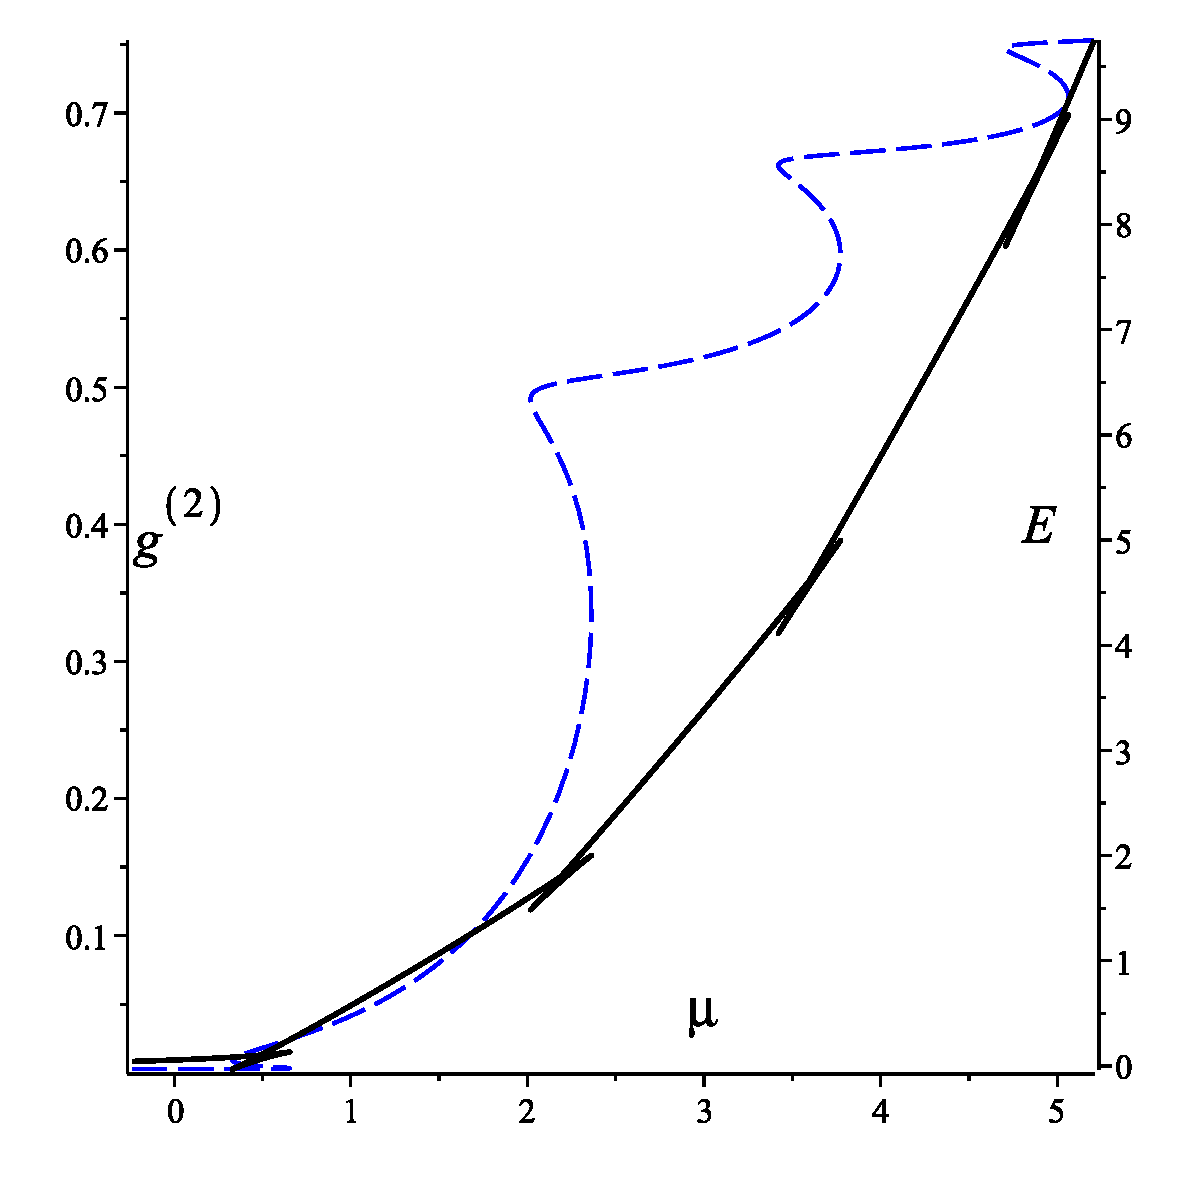
\includegraphics[width=0.6\textwidth,angle=0]{g2_vs_E_vs_mu}
	\caption{Pair distribution function $g^{(2)}$ along with quantity $E_0$ versus chemical potential $\beta\mu$. The temperature is $T^*=0.20$ (which is below the critical value).}
	\label{fig:g2_E_mu}
\end{figure}

